%%%%%%%%%%%%%%%%%%%%%%%%%%%%%%%%%%%%%%%%%%%%%%%%%%%%%%%%%%%%%%%%%%%%%%
%% Private Federated Aggregation of LLM-Agent Memory
%% Springer Nature LaTeX template (sn-jnl.cls, v3.1 Dec 2024)
%%
%% Build:  pdflatex -> bibtex -> pdflatex -> pdflatex
%% (or:    latexmk -pdf qpriviot-memory.tex)
%%
%% Figures live outside paper/ (see \graphicspath) so the notebook and the
%% paper share one copy: scripts/agentmem/rerun_figures.py regenerates them.
%%%%%%%%%%%%%%%%%%%%%%%%%%%%%%%%%%%%%%%%%%%%%%%%%%%%%%%%%%%%%%%%%%%%%%

% sn-mathphys-num = numbered citations, math/physical sciences.
% Single-column (sn-jnl default) for peer review; drop `iicol` was the
% two-column journal look. Re-add `iicol` only for a two-column proof.
\documentclass[pdflatex,sn-mathphys-num,12pt]{sn-jnl}

\usepackage{graphicx}%
\usepackage{multirow}%
\usepackage{amsmath,amssymb,amsfonts}%
\usepackage{amsthm}%
\usepackage{mathrsfs}%
\usepackage[title]{appendix}%
\usepackage{xcolor}%
\usepackage{textcomp}%
\usepackage{manyfoot}%
\usepackage{booktabs}%
\usepackage{algorithm}%
\usepackage{algorithmicx}%
\usepackage[noend]{algpseudocode}%
\usepackage{siunitx}%

\theoremstyle{thmstyleone}%
\newtheorem{theorem}{Theorem}%
\newtheorem{proposition}[theorem]{Proposition}%

\theoremstyle{thmstyletwo}%
\newtheorem{example}{Example}%
\newtheorem{remark}{Remark}%

\theoremstyle{thmstylethree}%
\newtheorem{definition}{Definition}%

\graphicspath{{../figures/}{figures/}}

% Shorthands for symbols the paper uses constantly.
\newcommand{\eps}{\varepsilon}
\newcommand{\R}{\mathbb{R}}
\newcommand{\Z}{\mathbb{Z}}
\newcommand{\norm}[1]{\left\lVert #1 \right\rVert}
\newcommand{\secref}[1]{\S\ref{#1}}

% Compact "x +- y" cells.
\newcommand{\pmm}[2]{$#1 \pm #2$}

% This paper is float-dense (20 tables, 6 figures, 1 algorithm). With LaTeX's stock
% parameters the queue congests and tall floats get deferred to the end of the
% document; these let a float take more of a page and let more of them sit together.
\setcounter{topnumber}{3}
\setcounter{bottomnumber}{2}
\setcounter{totalnumber}{5}
\renewcommand{\topfraction}{0.9}
\renewcommand{\bottomfraction}{0.7}
\renewcommand{\textfraction}{0.07}
\renewcommand{\floatpagefraction}{0.75}

\raggedbottom

\begin{document}

\title[Private Federated Aggregation of LLM-Agent Memory]{Private Federated
Aggregation of LLM-Agent Memory: Usable Shared Memory with a Measurable
Leakage-Drop Guarantee under Secure Aggregation and the Skellam Mechanism}

%%=====================================================================%%
%% TITLE PAGE: PPNA requires each author's full affiliation             %%
%% (Department, Institution, City, State, Country) and, if available,   %%
%% a 16-digit ORCID. The affiliation below is a placeholder             %%
%% ("Independent Researcher") so the document typesets with no dangling %%
%% superscript. BEFORE SUBMITTING: fill \orgdiv / \orgname / \city /    %%
%% \state / \country with the real address, and add \orcid{...} to the  %%
%% \author line (register free at https://orcid.org if you have none).  %%
%%=====================================================================%%
% First Author
\author*[1]{\fnm{Nikhil} \sur{Sharma}}\email{nikhilmsha@gmail.com}

% Second Author
\author[2]{\fnm{A. R.} \sur{Rajeswari}}\email{arrajeswari.2015@gmail.com}

% Affiliations
\affil*[1]{\orgname{MS in Software Engineering Student}, \orgaddress{\city{San Jose}, \state{CA}, \country{USA}\\ (ORCID: 0000-0002-1651-0879)}}

\affil[2]{\orgdiv{Director}, \orgname{ARR Shine Academy Pvt. Ltd.}, \orgaddress{\city{Madurai}, \country{India}}}
% Update at proof stage if the affiliation changes; keep the corresponding
% \email a stable personal address (not an institutional one) across any move.

%% Springer style: no cross-references, citations or equations in the abstract.
%% Abstract kept within the PPNA limit (150--250 words), no citations or
%% cross-references, per the journal's Instructions for Authors.
\abstract{Large Language Model (LLM) agents accumulate per-user memory (distilled notes and preferences) that makes them personal. Pooling it across users would give a fleet a shared \textbf{routing prior}, but memory is exactly the sensitive artifact: published extraction and membership-inference attacks recover verbatim user facts. We aggregate per-user memory-note embeddings into a bucketed \textbf{centroid memory} under \textbf{Secure Aggregation} composed with the discrete \textbf{Skellam mechanism}, so the pool carries a central differential-privacy (DP) guarantee with no trusted curator and no note in the clear. We evaluate on real long-horizon conversational memory and LLM-distilled agent notes, reading utility and leakage at the same operating point. Four findings. First, on a \textbf{joint frontier} measuring both axes at every bucket fidelity, the coarse regime offers strong utility with rigorous privacy guarantees: the pool keeps \textbf{95\% of clean retrieval utility} while a calibrated likelihood-ratio attack falls from an Area Under the Curve (AUC) of 0.833 to the 1\% false-positive floor. Second, that endpoint is \textbf{invisible to the weak attack the literature defaults to}: an uncalibrated cosine proxy reports chance on the release the calibrated attack breaks, so a proxy-only evaluation fails to detect leakage identified by calibrated LiRA evaluation. Third, \textbf{data-dependent preprocessing silently inflates such results}: fitting the projection on user notes is an unaccounted release that also manufactures an apparent dimension effect, gone under a public-seed projection. Fourth, we account for the \textbf{repeated release} a deployment requires, whose cost grows only as the square root of the round count. Every parameter of the mechanism is public or DP-accounted, so the reported budget covers the whole pipeline.}

\keywords{Differential privacy, Secure aggregation, Skellam mechanism,
LLM agent memory, Federated learning, Membership inference}

\maketitle



\section{Introduction}\label{sec:intro}

\paragraph{Agent memory is the new sensitive payload.} Production Large Language Model (LLM)-agent frameworks such as A-MEM~\cite{xu2024amem} and Mem0~\cite{chhikara2024mem0} persist a per-user store of distilled notes: ``the user is allergic to penicillin,'' ``prefers metric units,'' ``is migrating a Postgres 14 cluster.'' This memory is what makes an agent personal, and it is also a dense concentrate of personally identifying information. A natural, high-value idea is to \textbf{share memory across users}, so that a fleet of agents can profit from what the fleet collectively knows. But na\"ively pooling raw notes is a privacy disaster, and recent work shows the threat is concrete: \textbf{MEXTRA}~\cite{wang2025mextra} extracts verbatim memory content, and \textbf{MRMMIA}~\cite{chen2026mrmmia} performs membership inference against agent memory with high success.

\paragraph{Why the obvious defenses are insufficient.} Access-control layers (\emph{Collaborative Memory}~\cite{rezazadeh2025collabmem}) and on-device masking (\emph{MemPrivacy}~\cite{chen2026memprivacy}) restrict \emph{who} sees a note but provide no formal guarantee over the \emph{aggregate}, and a curated central datastore~\cite{abouelenein2026dpdatastore} reintroduces a trusted party. What is missing is a mechanism that (a) needs \textbf{no trusted curator}, (b) gives a \textbf{central-DP guarantee over the shared pool}, and (c) is shown to actually \textbf{degrade the known attacks} while keeping the pool useful.

\paragraph{Our approach.} We treat federated memory aggregation as a \textbf{secure summation of per-user bucketed embeddings}. Each user projects their notes to a working dimension $d$ with a \textbf{public-seed random projection}, maps them into $K$ shared buckets (random-hyperplane Locality-Sensitive Hashing (LSH)), forms a per-bucket sum-vector, and contributes it through \textbf{SecAgg}~\cite{bonawitz2017secagg} so the server sees only the masked sum; the \textbf{Skellam mechanism}~\cite{agarwal2021skellam} adds calibrated discrete noise that \textbf{composes under summation}, yielding a single distributed-DP guarantee on the pooled centroid memory. Retrieval is cosine lookup against the noised centroids. The cryptographic path is used \textbf{verbatim} from federated discrete-DP work; the novelty is the \emph{payload} (agent-memory embeddings) and the \emph{evaluation} (a measured attack-success drop).

\paragraph{Why this payload, and why now.} Federated DP for LLM adaptation is saturated, and recent federated-privacy work for LLMs targets other objects: DP synthetic-data generation (POPri~\cite{hou2025popri}) and privacy-constrained agent self-evolution (Fed-SE~\cite{chen2025fedse}). Contemporaneous agent-memory security surveys~\cite{lin2026survey} catalogue attacks and access-control defenses but no curator-free DP aggregation mechanism. Federated agent-memory aggregation under SecAgg $+$ discrete Skellam DP is thus an open seam. Crucially, agent-memory objects are \textbf{genuinely tiny-dimensional and often already discrete}, the regime where the discrete Skellam mechanism is most efficient.

\subsection*{Contributions}

\begin{enumerate}
  \item \textbf{Federated private memory aggregation using SecAgg and Skellam DP}, yielding a curator-free central-DP shared routing prior.
  \item \textbf{Joint utility--leakage evaluation using calibrated LiRA}. We demonstrate a positive endpoint on the joint frontier where the pool keeps 95\% of clean retrieval utility while a calibrated attack falls to the 1\% false-positive floor.
  \item \textbf{Demonstration that cosine proxies and data-dependent PCA confound privacy evaluation}. The uncalibrated cosine proxy commonly used in the literature substantially underestimates leakage relative to calibrated evaluation, and data-dependent projection can manufacture an apparent dimension crossover.
  \item \textbf{Full accounting including preprocessing, clipping, and repeated release}. Every parameter is public or DP-accounted, and we evaluate the realistic cost of re-aggregating memory over a deployment's lifecycle.
\end{enumerate}

\section{Related Work}\label{sec:related}

\paragraph{Federated DP with secure aggregation and discrete noise.} Federated learning~\cite{mcmahan2017fedavg} trains on decentralised data without centralising it, and SecAgg~\cite{bonawitz2017secagg} lets a server compute a sum of client vectors without seeing any summand. To obtain a differential-privacy (DP) guarantee~\cite{dwork2014foundations} that composes under that sum without a trusted curator, discrete mechanisms are used, such as the \textbf{Skellam mechanism}~\cite{agarwal2021skellam}, which is closed under addition and efficient at low bit-width. Prior deployments target \textbf{gradient} payloads~\cite{kairouz2021ddgauss,abadi2016dpsgd}. We reuse this path \emph{verbatim} but change the payload to \textbf{agent-memory embeddings} and the objective to \textbf{retrieval}.

\paragraph{Privacy of LLM-agent memory.} Agent frameworks A-MEM~\cite{xu2024amem} and Mem0~\cite{chhikara2024mem0} persist distilled per-user memories. Their privacy is under active attack: \textbf{MEXTRA}~\cite{wang2025mextra} extracts memory content and \textbf{MRMMIA}~\cite{chen2026mrmmia} runs membership inference~\cite{shokri2017mia}. Defenses so far are \textbf{access control}~\cite{rezazadeh2025collabmem} and \textbf{on-device masking}~\cite{chen2026memprivacy}, neither giving an aggregate formal guarantee. We provide the missing mechanism-side guarantee and cite the attacks as our evaluation harness.

\paragraph{Federated retrieval / datastores.} \emph{DP Datastore Generation}~\cite{abouelenein2026dpdatastore} partitions data with locality-sensitive hashing and adds calibrated DP noise to each bucket's aggregate. However, it is \textbf{centralized and single-curator}, uses generic additive noise with no secure aggregation, and targets classification, not agent memory. Our approach provides a \textbf{federated, curator-free} release under \textbf{SecAgg} with the \textbf{Skellam} mechanism, using the agent-memory embedding payload.

\paragraph{Dimension dependence of DP.} That utility degrades with dimension under DP is classical~\cite{bassily2014erm,chen2022price}. \secref{sec:crossover} shows that the apparent \emph{coupled} crossover, in which dimension governs pre-DP \emph{leakage} and DP \emph{utility-retention} simultaneously, is an artifact of a data-dependent projection.

\section{Threat Model and Problem Setup}\label{sec:threat}

\paragraph{Parties.} $N$ users, each with a local agent holding a set of memory notes; an honest-but-curious aggregation server; and downstream agents that query the shared memory.

\paragraph{Goal.} Produce a single \textbf{shared memory pool} (a set of $K$ centroid embeddings) that any agent can query by cosine similarity to retrieve relevant knowledge contributed by the fleet, such that the pool carries a \textbf{central $(\eps, \delta)$-DP guarantee at user granularity} and no individual user's notes can be reconstructed or their membership inferred.

\paragraph{Trust / adversary.} No trusted curator: under SecAgg the server observes only the masked sum. The adversary is a recipient of the released pool. It mounts \textbf{Membership inference} (decide whether the user who owns a note $x$ contributed to the pool, measuring ROC-AUC) and \textbf{Extraction} (advantage in reconstructing an in-bucket member embedding from the centroid). We measure leakage over all buckets with a calibrated attack (\secref{sec:lira}), and additionally evaluate a low-count tail lens to connect with prior proxy-based attacks. 

\paragraph{Threat boundary.} Our adversary is \textbf{passive}. Active, colluding clients (e.g., poisoning) and participation metadata (who participated in a round) are explicitly out of scope. We specify mandatory participation with padded dummy payloads to address the latter, but do not measure it.

\paragraph{Utility.} For a query $q$, retrieval routes to the top-$k$ centroids by cosine; utility is whether the \emph{right} content is retrieved.

\section{Bucketed Centroid Memory}\label{sec:centroid}

Let each note $i$ of user $u$ have embedding $e_i \in \R^{D}$ from a sentence encoder. We reduce to a working dimension $d$ with a \textbf{public-seed Gaussian random projection}~\cite{achlioptas2003rp} $P \in \R^{D \times d}$, $P_{jk} \sim \mathcal{N}(0, 1/d)$, L2-normalize, and assign to one of $K$ buckets by random-hyperplane LSH~\cite{charikar2002simhash}: fix $K$ random anchors $a_1, \dots, a_K$ and set $\mathrm{bucket}(i) = \arg\max_k \langle e_i, a_k \rangle$. Both $P$ and the anchors are drawn from a \textbf{published seed and never touch user data}, so shipping them releases nothing.

Each user forms, per bucket $k$, a \textbf{sum-vector} $v_u[k] = \sum_{i : \mathrm{bucket}(i) = k} e_i$ and a \textbf{count} $c_u[k]$. The (non-private) shared centroid is:

\begin{equation}\label{eq:centroid}
  \mu[k] \;=\; \mathrm{normalize}\!\left(
    \frac{\sum_u v_u[k]}{\sum_u c_u[k]}
  \right).
\end{equation}

Retrieval for query $q$ returns the top-$k$ buckets by $\cos(q, \mu[k])$.

\section{Private Release: SecAgg + Skellam}\label{sec:release}

\subsection{Clipping, quantisation, and sensitivity}\label{sec:clipping}

A user's contribution to the release is the \emph{whole} payload: the concatenation $V_u = [v_u[1]; \dots; v_u[K]] \in \R^{K \cdot d}$. We clip $V_u$ \textbf{globally}, to a single L2 bound $C$, and only then quantise to integers on a fixed grid of resolution $s = \texttt{range\_max} / B$ ($\texttt{range\_max} = 10^{6}$, $B$ the quantiser bound). This yields integer vectors amenable to SecAgg and discrete noise, with \textbf{user-level L2 sensitivity exactly $\Delta_2 = C \cdot s$}. (Two datasets are neighbours if one is obtained from the other by \textbf{adding or removing a single user}.)

\subsection{The clip bound must be public}\label{sec:clip}

$C$ and $B$ must not be derived directly from the private corpus without accounting.
\textbf{$B := C$ is free.} Since every note is L2-unit and the payload is clipped first, $|V_u[j]| \leq \norm{V_u}_2 \leq C$ for every coordinate $j$.
\textbf{$C$ is DP-selected.} We choose $C$ from a public geometric grid with the exponential mechanism~\cite{mcsherry2007expmech} on the rank utility $u(c) = -\left| \#\{u : \norm{V_u}_2 \leq c\} - 0.95 N \right|$. The sensitivity is:
\begin{equation}\label{eq:clip-sens}
      \Delta u \;=\; \max(1 - q,\; q) \;=\; q \;=\; 0.95 \;\leq\; 1,
    \end{equation}
We spend $\eps_c = 0.1$, which costs \textbf{0.2\% of the budget} ($\eps\ 9.29 \to 9.31$). The selection is conservative, biasing $C$ upward, meaning it only ever \emph{adds} noise.

Each user adds Skellam noise (a difference of two Poissons) to their quantised vector and submits it through \textbf{SecAgg}, so the server recovers only $\sum_u (\mathrm{quantise}(\mathrm{clip}(v_u)) + \mathrm{Skellam})$. The sum of independent Skellams is Skellam, meaning the \emph{released sum} carries the target noise with \textbf{no trusted curator}. 

\subsection{Vector-only release}\label{sec:vector-only}

Releasing \textbf{two} channels (the sum-vector and the counts) costs two RDP compositions. For the \emph{direction} of the retrieval centroid, normalisation cancels the count. Releasing \textbf{only the summed vector} yields identical retrieval at \textbf{${\sim}1.5\times$ tighter $\eps$}. The count channel's one non-redundant use is \emph{occupancy} (identifying empty buckets), but as detailed in Appendix~\ref{sec:app-occupancy}, no occupancy rule is simultaneously free and accurate.

\subsection{Privacy accounting}\label{sec:accounting}

We account with the exact discrete Skellam guarantee~\cite{agarwal2021skellam}, converting to $(\eps,\delta)$ through R\'enyi DP~\cite{mironov2017rdp}:
\begin{equation}\label{eq:skellam-rdp}
\begin{split}
  \eps_{\mathrm{RDP}}(\alpha) \;\leq\;
  &\frac{\alpha \Delta_2^2}{2\mu} \\[2pt]
  &{}+\; \min\!\left\{
    \frac{(2\alpha - 1)\Delta_2^2 + 6\Delta_1}{4\mu^2},\;
    \frac{3\Delta_1}{2\mu}
  \right\},
\end{split}
\end{equation}
with $\mu$ the per-coordinate released variance, $\Delta_2 = C s$, and $\Delta_1 \leq \sqrt{K d} \cdot \Delta_2$. We set $\delta = 10^{-5}$. 

\begin{table*}[t]
  \centering
  \caption{$\sigma \to \eps$ at the $K = 32$, $d = 32$ operating point
  ($\delta = 10^{-5}$). Every $\eps$ is the \emph{total}: the Skellam release plus the
  $\eps_c = 0.1$ spent DP-selecting the clip bound (\secref{sec:clip}). The projection
  and $B := C$ contribute nothing. The ``classic'' column is the label the exploration
  grid was run under and is \emph{invalid} for $\eps > 1$; it is shown only to map the
  run labels onto the rigorous budgets. $\sigma$ is given to four decimals because each
  $\eps$ is computed at the \emph{exact} $\sigma$ the grid was run at
  ($\sigma = \sqrt{2\ln(1.25/\delta)}\,/\,\text{label}$); rounding $\sigma$ to three
  decimals first shifts the budget by ${\sim}0.01$.}
  \label{tab:sigma-eps}
  \begin{tabular}{@{}lrrr@{}}
    \toprule
    & \multicolumn{1}{c}{classic label} & \multicolumn{2}{c@{}}{Skellam-RDP (exact)} \\
    \cmidrule(l){2-2}\cmidrule(l){3-4}
    $\sigma$ & (invalid, $\eps > 1$) & \textbf{vector-only (1 rel.)} & two-channel (2 rel.) \\
    \midrule
    0.3028 & 16.00 & 22.13 & 33.34 \\
    0.6056 &  8.00 & \textbf{9.31} & 13.95 \\
    1.6149 &  3.00 & \textbf{3.21} &  4.63 \\
    2.8540 &  1.70 & \textbf{1.81} &  2.56 \\
    \bottomrule
  \end{tabular}
\end{table*}

\subsection{The full mechanism}\label{sec:algorithm}

Algorithm~\ref{alg:main} defines the end-to-end procedure. Detailed implementation constraints (modular field size, mandatory participation padding, and client dropout handling) are discussed in Appendices \ref{sec:app-constraints} and \ref{sec:app-dropout}.

\begin{algorithm*}[t]
\caption{Private Federated Memory Aggregation (SecAgg $+$ Skellam, vector-only
release). Public/shared parameters are as listed in the text above.}
\label{alg:main}
\footnotesize
\begin{algorithmic}[1]
  \Statex \textbf{\textsc{Server, once}} \hfill \emph{(public parameters; \secref{sec:clip})}
  \State $C \gets \textsc{ExpMech}_{\eps_c}\big(\text{grid},\,
         u(c) = -|\#\{u : \norm{V_u}_2 \leq c\} - 0.95 N|\big)$
         \Comment{DP-selected clip}
  \State $B := C$; \; $s \gets \texttt{range\_max}/B$; \;
         $\mu \gets (\sigma C s)^2$
         \Comment{$|\text{coord}| \leq \norm{V_u}_2 \leq C$}

  \Statex
  \Statex \textbf{\textsc{Client} $u$} \hfill \emph{(local; note text never leaves the device)}
  \For{each note $i$ of user $u$}
    \State $e_i \gets \mathrm{normalize}\big(P(\mathrm{Encoder}(\text{note}_i))\big)$
           \Comment{$384\text{-d} \to d$, L2-unit}
    \State $b(i) \gets \arg\max_k \langle e_i, a_k \rangle$
           \Comment{LSH bucket}
  \EndFor
  \State $v_u[k] \gets \sum_{i : b(i) = k} e_i$ \; for $k = 1 \dots K$
         \Comment{per-bucket sum-vector}
  \State $V_u \gets [\,v_u[1]; \dots; v_u[K]\,] \in \R^{K d}$
         \Comment{the user's \textsc{full} payload}
  \State $V_u \gets V_u \cdot \min\!\big(1,\, C / \norm{V_u}_2\big)$
         \label{alg:global-clip}
         \Comment{\textbf{global} clip $\Rightarrow \Delta_2 = C s$ (\secref{sec:app-constraints})}
  \For{each bucket $k = 1 \dots K$}
    \State $z_u[k] \gets \mathrm{round}\big(v_u[k] \cdot s\big) \in \Z^{d}$
           \Comment{quantise; $B := C$ never clips}
    \State $\tilde n_u[k] \gets \mathrm{Skellam}(\mu / M_{\min})$
           \label{alg:noise}
           \Comment{noise share, sized to survivors}
    \State $\tilde z_u[k] \gets z_u[k] + \tilde n_u[k]$
           \Comment{DP noise, in the integer domain}
    \State $m_u[k] \gets \tilde z_u[k] + \mathrm{mask}_u[k]$, \;
           $\textstyle\sum_u \mathrm{mask}_u[k] = 0$
           \Comment{SecAgg zero-sum mask}
  \EndFor
  \State \textbf{submit} $\{m_u[k]\}_{k=1}^{K}$ to the server

  \Statex
  \Statex \textbf{\textsc{Server}} \hfill \emph{(honest-but-curious; sees only masked sums)}
  \State \textbf{if} fewer than $M_{\min}$ clients survive \textbf{then abort}
  \For{each bucket $k = 1 \dots K$}
    \State $S[k] \gets \sum_{u \,\mathrm{alive}} m_u[k]
           = \sum_u z_u[k] + \mathrm{Skellam}\big(\tfrac{M}{M_{\min}}\mu\big)$
           \Comment{masks cancel}
    \State $\tilde\mu[k] \gets \mathrm{normalize}\big(S[k] / s\big)$
           \label{alg:normalize}
           \Comment{\textbf{every} bucket; no occupancy oracle (\secref{sec:vector-only})}
  \EndFor
  \State \textbf{release} the private centroid memory $\{\tilde\mu[k]\}_{k=1}^{K}$

  \Statex
  \Statex \textbf{\textsc{Retrieval}} \hfill \emph{(any downstream agent, query $q$)}
  \State \textbf{return} top-$k$ buckets by $\cos\big(\mathrm{normalize}(P(\mathrm{Encoder}(q))),\,
         \tilde\mu[k]\big)$ over $\{k : \tilde\mu[k] \neq 0\}$

  \Statex
  \Statex \textbf{\textsc{Accounting}} \hfill \emph{(\secref{sec:accounting}, exact Skellam-RDP)}
  \State $\Delta_2 \gets C s$; \; $\Delta_1 \gets \sqrt{K d}\,\Delta_2$
         \Comment{over the full $Kd$ payload; valid \emph{because} line~\ref{alg:global-clip} clips globally}
  \State $\eps_{\mathrm{RDP}}(\alpha) = \frac{\alpha \Delta_2^2}{2\mu}
         + \min\!\big\{\frac{(2\alpha - 1)\Delta_2^2 + 6\Delta_1}{4\mu^2},
                       \frac{3\Delta_1}{2\mu}\big\}
         + \frac{\alpha \eps_c^2}{2}$
         \Comment{last term: DP clip selection}
  \State $\eps \gets \min_\alpha \big[\eps_{\mathrm{RDP}}(\alpha) + \ln(1/\delta)/(\alpha - 1)\big]$
         \Comment{1 release $\Rightarrow {\sim}1.5\times$ tighter $\eps$}
\end{algorithmic}
\end{algorithm*}

\section{Experimental Setup}\label{sec:setup}

\paragraph{Datasets} (1) \textbf{LongMemEval (oracle)}~\cite{wu2024longmemeval}: real long-horizon conversational memory (500 users, 10,957 note embeddings). (2) \textbf{LongMemEval (\texttt{s})}: full-haystack variant (246,073 notes) for at-scale checks. (3) \textbf{LLM-distilled notes} (A-MEM/Mem0-style): 6,116 distilled notes, the realistic payload. (4) \textbf{Synthetic controls}: 20-Newsgroups.

\paragraph{Embeddings} \texttt{all-MiniLM-L6-v2} (384-d)~\cite{reimers2019sbert}, reduced to $d$ by a \textbf{public-seed Gaussian random projection}.

\paragraph{Mechanism \& Protocol} We use the faithful crypto path. The clip bound $C$ is DP-selected ($\eps_c = 0.1$). We report 5-seed means $\pm$ std for utility and 3-seed $\times$ 48 shadow releases for the calibrated LiRA.

\section{Results}\label{sec:results}

Every $\eps$ value is the rigorous Skellam-RDP label, covering the whole pipeline including the clip-bound selection. 

\subsection{The joint frontier: both axes, one operating point}\label{sec:frontier}

We measure utility \emph{and} the calibrated LiRA attack at every $K$, reporting the \textbf{joint frontier} (Table~\ref{tab:frontier}, Fig.~\ref{fig:joint-frontier}a).

\begin{table*}[t]
  \centering
  \caption{\textbf{The joint frontier}: retrieval utility and \emph{calibrated} leakage
  at the \textbf{same} $K$ (LongMemEval-oracle, $d = 32$, vector-only; utility 5-seed,
  LiRA 3-seed $\times$ 48 shadows). Leakage is the offline-LiRA of \secref{sec:lira},
  not the cosine proxy; as \secref{sec:proxy-blind} shows, that proxy reports chance at
  exactly the $K$ one would deploy. TPR@1\%FPR floor $= 0.010$.}
  \label{tab:frontier}
  \footnotesize
  \setlength{\tabcolsep}{2.5pt}
  \begin{tabular}{@{}lrll r rr rr rr@{}}
    \toprule
    & & \multicolumn{3}{c}{utility (evidence-recall@5)}
      & \multicolumn{2}{c}{LiRA AUC} & \multicolumn{2}{c}{TPR@1\%FPR}
      & \multicolumn{2}{c@{}}{decode-extract} \\
    \cmidrule(lr){3-5}\cmidrule(lr){6-7}\cmidrule(lr){8-9}\cmidrule(l){10-11}
    $K$ & Chance & Clean & $\eps \approx 9.3$ & Reten. & clean & $\eps 9.3$
        & clean & $\eps 9.3$ & clean & $\eps 9.3$ \\
    \midrule
    \textbf{32} & 0.156 & \pmm{0.428}{0.046} & \pmm{\mathbf{0.406}}{\mathbf{0.054}} & \textbf{95\%}
      & 0.833 & \textbf{0.502} & 0.175 & \textbf{0.011} & 0.771 & 0.396 \\
    64          & 0.078 & \pmm{0.320}{0.045} & \pmm{0.276}{0.049} & 86\%
      & 0.908 & 0.505 & 0.357 & 0.011 & 0.667 & 0.188 \\
    \textbf{128} & 0.039 & \pmm{0.233}{0.031} & \pmm{0.167}{0.039} & \textbf{72\%}
      & 0.954 & 0.502 & 0.552 & \textbf{0.011} & 0.794 & \textbf{0.070} \\
    256         & 0.020 & \pmm{0.167}{0.022} & \pmm{0.100}{0.035} & 60\%
      & 0.981 & 0.503 & 0.750 & 0.011 & 0.789 & 0.029 \\
    512         & 0.010 & \pmm{0.152}{0.026} & \pmm{0.062}{0.031} & 41\%
      & 0.993 & 0.505 & 0.874 & 0.013 & 0.874 & 0.007 \\
    1024        & 0.005 & \pmm{0.135}{0.017} & \pmm{0.032}{0.016} & 24\%
      & 0.997 & 0.504 & 0.945 & 0.013 & 0.912 & 0.003 \\
    2048        & 0.002 & \pmm{0.128}{0.013} & \pmm{0.016}{0.010} & 13\%
      & 0.998 & 0.505 & 0.957 & 0.012 & 0.928 & 0.001 \\
    \bottomrule
  \end{tabular}
\end{table*}

\begin{figure*}[t]
  \centering
  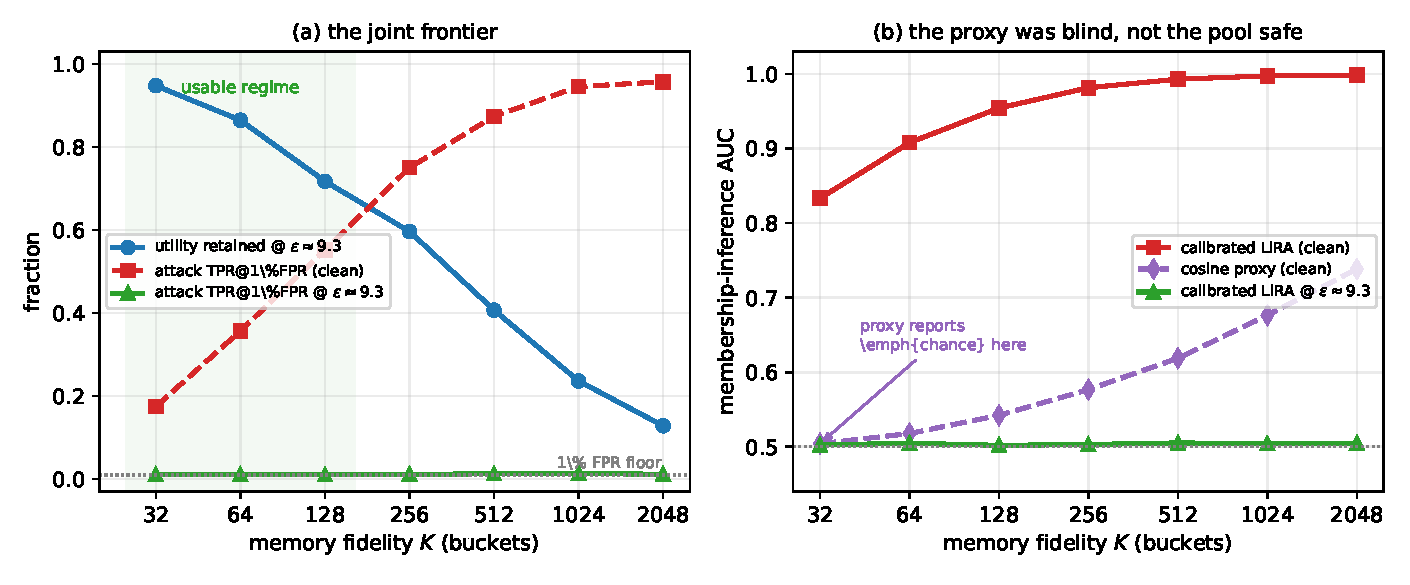
\includegraphics[width=\linewidth]{fig_joint_frontier.pdf}
  \caption{\textbf{(a) The joint frontier.} Utility retention falls monotonically with
  fidelity $K$ while clean leakage rises; DP pins the calibrated attack at the 1\%
  false-positive floor \emph{uniformly}, so the frontier is governed by the utility axis
  alone and the coarse-$K$ regime dominates. \textbf{(b) The proxy underestimates leakage where it
  matters.} The uncalibrated cosine proxy (purple) reports chance at $K = 32$ on
  the same clean release where the calibrated LiRA (red) reads AUC 0.833: the pool
  still exhibits leakage there (\secref{sec:proxy-blind})}
  \label{fig:joint-frontier}
\end{figure*}

\begin{enumerate}
  \item \textbf{The DP release reduces calibrated attack performance to near-chance levels at \emph{every} $K$.} LiRA AUC lands in $0.502$--$0.505$ and TPR@1\%FPR in $0.011$--$0.013$ for all fidelities, even as the \emph{clean} attack climbs to AUC $0.998$. The privacy axis is \textbf{flat}.
  \item \textbf{The operating point is set by retention.} Retention falls $95 \to 13\%$ as $K$ grows $32 \to 2048$. \textbf{$K = 32$ is the recommended point}: 95\% retention with the membership attack at the floor.
  \item \textbf{Closed-set reconstruction bound.} At $K = 32$, reconstruction-decode only halves ($0.771 \to 0.396$) against a chance floor of $0.010$. DP does not defeat closed-set reconstruction at the recommended point, although this metric is identical to utility and assumes the adversary already holds the notes.
\end{enumerate}

\subsection{Calibrated attack: LiRA membership inference}\label{sec:lira}

The uncalibrated cosine similarity score is actively misleading (\secref{sec:proxy-blind}). We run the \textbf{modern MIA standard}~\cite{carlini2022lira}: an \textbf{offline LiRA} testing with the per-target likelihood ratio across shadow releases.

\begin{table*}[t]
  \centering
  \caption{Calibrated offline-LiRA and reconstruction-decode extraction (LongMemEval oracle,
  $d = 32$, 3 seeds $\times$ 48 shadow releases). The clean release is far more leaky than the
  cosine proxy revealed, and DP still reduces the strong attack to near-chance levels on every axis at once.}
  \label{tab:lira}
  \begin{tabular}{@{}llrrrr@{}}
    \toprule
    $K$ & Release & AUC & TPR@1\%FPR & TPR@0.1\%FPR & Decode-extract \\
    \midrule
    1024 & clean               & 0.997          & \textbf{0.945} & 0.784 & 0.912 \\
    1024 & $\eps \approx 9.3$  & \textbf{0.504} & \textbf{0.013} & 0.001 & 0.003 \\
    1024 & $\eps \approx 3.2$  & 0.501          & 0.012          & 0.002 & 0.001 \\
    \bottomrule
  \end{tabular}
\end{table*}
\begin{table*}[t]
  \centering
  \caption{LiRA across the fidelity sweep. Clean leakage rises with $K$; DP pins every cell
  at the false-positive floor.}
  \label{tab:lira-sweep}
  \footnotesize
  \begin{tabular}{@{}lrrrr@{}}
    \toprule
    $K$ & Clean TPR@1\%FPR & $\eps \approx 9.3$ TPR@1\%FPR & Clean decode & $\eps \approx 9.3$ decode \\
    \midrule
    512  & 0.874 & 0.013 & 0.874 & 0.007 \\
    1024 & 0.945 & 0.013 & 0.912 & 0.003 \\
    2048 & 0.957 & 0.012 & 0.928 & 0.001 \\
    \bottomrule
  \end{tabular}
\end{table*}

Calibration exposes that on the clean pool an adversary re-identifies members at \textbf{${\approx}95\%$ true-positive rate at a 1\% false-positive budget}. The Skellam release drives the attack to \textbf{chance on every axis at once}. DP pins every cell at the false-positive floor across the fidelity sweep (Table~\ref{tab:lira-sweep}).

\subsection{The dimension crossover is a projection artifact}\label{sec:crossover}

Under a PCA projection \textbf{fit on the users' own notes}, growing $d$ appears to simultaneously raise pre-DP leakage and lower DP utility-retention. However, a data-fit PCA is an unaccounted release. When running with a \textbf{public-seed Gaussian projection} (\texttt{randproj}) or a disjoint public PCA, the effect vanishes (Tables~\ref{tab:abl-utility},~\ref{tab:abl-leakage}, Fig.~\ref{fig:projection-ablation}). 

\begin{table*}[t]
  \centering
  \caption{\textbf{Private utility} under the three projections
  (topic-acc @ $\eps \approx 9.3$, real \texttt{all-MiniLM-L6-v2}, $N = 100$, $K = 32$;
  higher is better). Tiny-$d$ wins \emph{only} under the leaky data-dependent PCA.}
  \label{tab:abl-utility}
  \begin{tabular}{@{}lrrr@{}}
    \toprule
    $d$ & data-PCA (leaky) & randproj (free) & publicPCA (free) \\
    \midrule
    \textbf{32}            & \textbf{0.308} & 0.151          & 0.147 \\
    64                     & 0.285          & \textbf{0.178} & 0.150 \\
    128                    & 0.240          & 0.158          & 0.142 \\
    384 \emph{(identity)}  & 0.161          & 0.161          & \textbf{0.161} \\
    \bottomrule
  \end{tabular}
\end{table*}
\begin{table*}[t]
  \centering
  \caption{\textbf{Leakage} under the three projections (tail-AUC at $K = 1024$;
  $0.5 =$ no leakage). The pre-DP gradient that motivated the crossover claim exists only
  under data-PCA; post-DP every cell is at chance.}
  \label{tab:abl-leakage}
  \begin{tabular}{@{}lrrrrr@{}}
    \toprule
    & \multicolumn{3}{c}{clean (pre-DP)} & \multicolumn{2}{c@{}}{$\eps \approx 9.3$} \\
    \cmidrule(lr){2-4}\cmidrule(l){5-6}
    $d$ & data-PCA & randproj & publicPCA & data-PCA & randproj \\
    \midrule
    32                    & 0.944 & 0.988 & 0.975 & 0.522 & 0.499 \\
    64                    & 0.969 & 0.991 & 0.985 & 0.513 & 0.500 \\
    128                   & 0.985 & 0.992 & 0.991 & 0.540 & 0.545 \\
    384 \emph{(identity)} & 0.989 & 0.989 & 0.989 & 0.541 & 0.541 \\
    \bottomrule
  \end{tabular}
\end{table*}
\begin{figure*}[t]
  \centering
  
\includegraphics[width=\linewidth]{fig_projection_ablation.pdf}
  \caption{The dimension crossover is a property of the projection, not of the
  mechanism. \textbf{(a)} Private utility: tiny-$d$ wins only under the
  data-dependent PCA; under either data-independent projection its advantage
  vanishes into the seed noise. \textbf{(b)} Pre-DP leakage: data-PCA shows the rising gradient the
  crossover claim rested on; the honest projections are saturated. All three
  converge at $d = 384$, where the projection \emph{is} the identity: the
  control. Shaded band: post-DP tail-AUC, flat at chance for every $d$ and every
  projection}
  \label{fig:projection-ablation}
\end{figure*}

Tiny-$d$ remains a reasonable engineering default ($12\times$ smaller payload) but it is not a privacy/utility free lunch. Data-dependent preprocessing is both an unaccounted release \emph{and} a confound that manufactures this dimension effect.

\subsection{The uncalibrated cosine proxy substantially underestimates leakage in the deployment-relevant regime}\label{sec:proxy-blind}

Comparing the uncalibrated cosine proxy to the calibrated attack (Fig.~\ref{fig:joint-frontier}b), at $K = 32$ the proxy reads \textbf{AUC 0.504} on the \emph{identical clean release} where the calibrated LiRA reads \textbf{AUC 0.833} and $17\times$-above-floor TPR. The proxy fails to detect leakage revealed by calibrated LiRA evaluation, and manufactures a false story that leakage is only a sparse, high-$K$ phenomenon.

\subsection{Distilled notes validation}\label{sec:distilled}

\begin{table*}[t]
  \centering
  \caption{\textbf{Calibrated} LiRA on the LLM-distilled payload (500 users, 6{,}116 notes,
  $K = 32$, $d = 32$; 3 seeds $\times$ 48 shadows): the realistic agent-memory object, measured
  with the attack \secref{sec:proxy-blind} shows to be the only trustworthy one. The raw-turn
  row is Table~\ref{tab:frontier}'s $K = 32$ row, repeated for comparison at the \emph{same}
  operating point.}
  \label{tab:distilled-lira}
  \small
  \begin{tabular}{@{}llrrr@{}}
    \toprule
    Payload & Release & AUC & TPR@1\%FPR & Decode-extract \\
    \midrule
    Raw dialogue turns          & clean              & 0.833 & 0.175 & 0.771 \\
    Raw dialogue turns          & $\eps \approx 9.3$ & 0.502 & \textbf{0.011} & 0.396 \\
    \midrule
    \textbf{LLM-distilled notes} & clean              & \textbf{0.838} & \textbf{0.171} & \textbf{0.750} \\
    \textbf{LLM-distilled notes} & $\eps \approx 9.3$ & 0.503 & \textbf{0.011} & \textbf{0.302} \\
    \bottomrule
  \end{tabular}
\end{table*}
\begin{figure}[t]
  \centering
  
\includegraphics[width=\columnwidth]{fig_distilled_utility.pdf}
  \caption{Distilled-notes utility (answer-recall@5). Density governs DP
  retention: the dense 500-user buckets ($K = 32$) retain \textbf{89\%} at
  $\eps \approx 9.3$, whereas the sparser 100-user pilot retains only 65\% at the
  same budget. More contributors per bucket $\Rightarrow$ cheaper DP}
  \label{fig:distilled-utility}
\end{figure}

We run the calibrated LiRA directly on the distilled pool (Table~\ref{tab:distilled-lira}). The clean distilled pool exhibits substantial measurable leakage, and the private release reduces attack performance to the floor. On the realistic agent-memory payload, the attack is defeated at the same operating point and budget as on raw turns.

\subsection{Accounting and repeated release}\label{sec:multiround}

The total $\eps$ decomposes cleanly (Table~\ref{tab:eps-decomp}). The clip bound selection costs 0.2\%, and the projection and discretisation are free.

\begin{table*}[t]
  \centering
  \caption{$\eps$ decomposition at $\sigma = 0.6056$, $\delta = 10^{-5}$, $K = 32$,
  $d = 32$. The reported budget covers the \emph{whole} pipeline, not just its last stage.}
  \label{tab:eps-decomp}
  \footnotesize
  \begin{tabular}{@{}lrl@{}}
    \toprule
    Term & $\eps$ & Note \\
    \midrule
    Continuous-Gaussian RDP reference   & 9.2909          & reference point \\
    $+$ discretisation (Skellam)        & 9.2909          & surcharge $1.3 \times 10^{-11}$: free at $\texttt{range\_max} = 10^{6}$ \\
    $+$ projection (public seed)        & 9.2909          & data-independent $\Rightarrow +0.000$ \\
    $+$ DP clip-bound selection ($\eps_c = 0.1$) & \textbf{9.3109} & \textbf{$+0.020$ (0.2\%)} \\
    \bottomrule
  \end{tabular}
\end{table*}
\begin{table*}[t]
  \centering
  \caption{Buying a re-aggregation cadence inside a \textbf{fixed} total budget
  ($\eps = 9.31$, $K = 32$, $d = 32$, $\delta = 10^{-5}$; clip bound selected once,
  publicly). $\sigma$ is solved from the Skellam-RDP accountant at $T$ releases;
  retention is measured at that $\sigma$ (5 seeds), not extrapolated. The last column is
  what those $T$ releases would \emph{actually} have cost had we kept the single-shot
  $\sigma = 0.606$ and simply re-released, i.e.\ the budget an unaccounted deployment
  would silently be spending.}
  \label{tab:multiround}
  \begin{tabular}{@{}rlrrrr@{}}
    \toprule
    $T$ & cadence & $\sigma$ needed & recall@5 & Retention & naive $\eps$ \\
    \midrule
    1  & single shot (this paper) & 0.606 & 0.406 & \textbf{95\%} & 9.3 \\
    4  & quarterly, 1 year        & 1.211 & 0.382 & 89\% & 22.1 \\
    \textbf{12} & \textbf{monthly, 1 year} & 2.098 & 0.349 & \textbf{81\%} & 44.2 \\
    30 & daily, 1 month           & 3.317 & 0.313 & 73\% & 93.3 \\
    52 & weekly, 1 year           & 4.367 & 0.283 & 66\% & 153.3 \\
    \bottomrule
  \end{tabular}
\end{table*}

A deployed memory is re-aggregated as users write notes. Re-releasing $T$ times at the single-shot noise scale rapidly depletes the budget. However, because the required $\sigma$ grows only as $\sqrt{T}$, a cadence can be bought up front: a pool re-aggregated \textbf{monthly for a full year} fits inside the \textbf{same $\eps \approx 9.3$} at 81\% retention (Table~\ref{tab:multiround}).

\section{Discussion and Limitations}\label{sec:discussion}

\subsection{Strengths}
\textbf{Membership protection.} The clean pool leaks at every fidelity, and DP pins the calibrated attack at the false-positive floor uniformly. The privacy axis is flat in $K$, separating the privacy guarantee from the utility tuning.

\textbf{Calibrated evaluation.} The analysis demonstrates the limitations of standard uncalibrated proxies and data-dependent projections, revealing the true leakage of the status-quo and validating the mechanism under a stronger lens.

\textbf{Full accounting.} The mechanism bounds the whole pipeline, including data-independent projection, DP clip-bound selection, and repeated lifecycle releases.

\subsection{Limitations}
\textbf{Open-set inversion not evaluated.} Open-set embedding inversion remains untested and is an important direction for future work. While membership is driven to chance, \emph{closed-set} reconstruction is not (\secref{sec:frontier}).

\textbf{Active adversaries not evaluated.} Our adversary is passive. Robust aggregation against poisoning from active, colluding clients is an orthogonal open problem.

\textbf{Benchmark limitations.} The pool is a routing prior, not a note exchange. We evaluate routing fidelity, but LongMemEval is a personal-recall benchmark where cross-user knowledge does not naturally transfer. 

\subsection{Future Work}
Future research should explore downstream task-transfer benchmarks to validate the end-to-end performance gains of a shared routing prior, and evaluate the mechanism's robustness against active adversaries or longitudinal drift in real deployments.

\section{Conclusion}\label{sec:conclusion}

LLM agents accumulate per-user memory that makes them personal but contains sensitive information. Pooling this memory across users can provide a shared routing prior for the fleet, but naively sharing it can expose verbatim facts to extraction and membership-inference attacks. We addressed this problem by aggregating per-user memory-note embeddings into a bucketed centroid memory under Secure Aggregation composed with the discrete Skellam mechanism, ensuring that the pool carries a central differential-privacy (DP) guarantee with no trusted curator.

Our main finding is that on a joint frontier measuring utility and leakage, the coarse-fidelity regime is both offering strong utility with rigorous privacy guarantees. At $K = 32$, the pool retains 95\% of clean retrieval utility while a calibrated likelihood-ratio attack falls to the 1\% false-positive floor, a result that holds on realistic LLM-distilled agent memory payloads. Consistent with the findings of Section \ref{sec:crossover} and \ref{sec:proxy-blind}, evaluating this regime requires calibrated attacks and public-seed projections, as uncalibrated proxies and data-dependent projections substantially underestimate leakage and introduce confounding effects.

Open-set embedding inversion remains untested and is an important direction for future work. Additionally, future research should explore downstream task-transfer benchmarks to validate the end-to-end performance gains of a shared routing prior, as well as evaluate the mechanism's robustness against active adversaries and poisoning in real-world, multi-round deployments.

\begin{appendices}
\section{Implementation Constraints}\label{sec:app-constraints}
\emph{Modular field size.} SecAgg sums in a finite field $\Z_p$. At our operating point, a prime $p > 10^{9}$ is sufficient. The reference implementation uses \texttt{int64}.
\emph{Mandatory participation.} A client with no new notes must submit an all-zero payload with Skellam noise and a mask, ensuring uniform participation indistinguishable from active clients.
\emph{Global clipping cross-bucket sensitivity.} Clipping each bucket separately would yield sensitivity $\sqrt{b_u} \cdot C$ (where $b_u$ is buckets touched). We clip \textbf{globally}, so the full payload sensitivity remains $C$.

\section{Client Dropout}\label{sec:app-dropout}
If $N$ clients inject $\mathrm{Skellam}(\mu/N)$ but only $M < N$ survive, the effective noise drops and the guarantee degrades (Table~\ref{tab:dropout}). We specify calibrating noise to a survival floor $M_{\min}$ (Algorithm~\ref{alg:main}) or using fault-tolerant noise reconstruction.

\begin{table*}[t]
  \centering
  \caption{Client dropout silently breaks the guarantee. True $\eps$ realised when
  each of $N$ clients injects a naive $\mu/N$ noise share but only $M$ survive.}
  \label{tab:dropout}
  \begin{tabular}{@{}lrrrrr@{}}
    \toprule
    survivors $M/N$ & 1.00 & 0.90 & 0.70 & 0.50 & 0.25 \\
    \midrule
    true $\eps$ (nominal $\eps \approx 9.31$) & 9.31 & 9.92 & 11.61 & \textbf{13.95} & \textbf{22.13} \\
    true $\eps$ (nominal $\eps \approx 3.21$) & 3.21 & 3.39 &  3.87 & \textbf{4.63}  & \textbf{6.74}  \\
    \bottomrule
  \end{tabular}
\end{table*}

\section{Occupancy Channel}\label{sec:app-occupancy}
Normalisation turns a pure-noise empty bucket into a unit vector. At $K \leq 256$, empty buckets are rare (Table~\ref{tab:occupancy-rate}). If detected, the binary user-indicator channel is the optimal privacy strategy but still costs a full second composition (Table~\ref{tab:occupancy-detect}). No rule is simultaneously free and accurate, as occupancy and membership are the same signal.

\begin{table*}[t]
  \centering
  \caption{Empty-bucket rate by fidelity $K$ (5 anchor seeds). Every retrieval number in
  this paper is reported at $K \leq 256$, where at most one bucket of 256 is ever empty.}
  \label{tab:occupancy-rate}
  \footnotesize
  \setlength{\tabcolsep}{3pt}
  \begin{tabular}{@{}lrrrrrrr@{}}
    \toprule
    $K$ & 32 & 64 & 128 & 256 & 512 & 1024 & 2048 \\
    \midrule
    Empty buckets (\%)
      & \textbf{0.00} & \textbf{0.00} & \textbf{0.00}
      & \pmm{0.23}{0.19} & \pmm{2.66}{0.88} & \pmm{10.14}{1.53} & \pmm{22.91}{2.01} \\
    \bottomrule
  \end{tabular}
\end{table*}
\begin{table*}[t]
  \centering
  \caption{Occupancy-detection AUC (empty vs occupied; $0.5 =$ undetectable), against the total
  $\eps$ of the release. No rule is simultaneously free and accurate.}
  \label{tab:occupancy-detect}
  \small
  \setlength{\tabcolsep}{4pt}
  \begin{tabular}{@{}llrrrr@{}}
    \toprule
    Occupancy rule & Sens.\ $C_c$ & $\eps$ & $K = 512$ & $K = 1024$ & $K = 2048$ \\
    \midrule
    $\norm{S[k]}$ vs floor $\sigma C \sqrt{d}$ (free: post-proc.) & n/a & \textbf{9.31} & 0.524 & 0.479 & 0.490 \\
    Raw-count, $\sigma_c = 2$ (cheap 2nd comp.)                   & 20.2 & 9.81 & 0.695 & 0.561 & 0.550 \\
    \textbf{User-indicator}, $\sigma_c = 2$                       & 9.7--12.4 & 9.81 & 0.723 & 0.593 & 0.549 \\
    Raw-count, $\sigma_c = \sigma_v$ (full 2nd comp.)             & 20.2 & 13.95 & 0.824 & 0.683 & 0.633 \\
    \textbf{User-indicator}, $\sigma_c = \sigma_v$                & 9.7--12.4 & 13.95 & \textbf{0.873} & \textbf{0.764} & \textbf{0.698} \\
    \bottomrule
  \end{tabular}
\end{table*}

\section{At-Scale Generality}\label{sec:app-at-scale}
On the full LongMemEval \texttt{s} variant (246k notes), utility retention is 97--100\% (Table~\ref{tab:at-scale-utility}). The low-count tail vanishes (Table~\ref{tab:at-scale-leakage}), meaning DP costs nothing measurable on retrieval at scale.

\begin{table*}[t]
  \centering
  \caption{At-scale utility (LongMemEval \texttt{s}, 246k notes; evidence-recall@5,
  $d = 32$, 5-seed).}
  \label{tab:at-scale-utility}
  \begin{tabular}{@{}lrlll r@{}}
    \toprule
    $K$ & Chance & Clean & $\eps \approx 9.3$ & $\eps \approx 3.2$ & Retention@$\eps \approx 9.3$ \\
    \midrule
    \textbf{32} & 0.156 & \pmm{0.422}{0.056} & \pmm{0.421}{0.059} & \pmm{0.422}{0.058} & \textbf{100\%} \\
    64          & 0.078 & \pmm{0.309}{0.041} & \pmm{0.312}{0.041} & \pmm{0.301}{0.037} & \textbf{101\%} \\
    128         & 0.039 & \pmm{0.223}{0.023} & \pmm{0.218}{0.023} & \pmm{0.201}{0.027} & \textbf{98\%} \\
    256         & 0.020 & \pmm{0.159}{0.020} & \pmm{0.154}{0.018} & \pmm{0.134}{0.022} & \textbf{97\%} \\
    \bottomrule
  \end{tabular}
\end{table*}
\begin{table*}[t]
  \centering
  \caption{At-scale leakage (LongMemEval \texttt{s}). The vulnerable tail all but vanishes, and
  membership inference is at chance even on the clean pool.}
  \label{tab:at-scale-leakage}
  \begin{tabular}{@{}lrrr@{}}
    \toprule
    $K$ & Low-count tail \% & Clean all-AUC & $\eps \approx 9.3$ all-AUC \\
    \midrule
    512  & 0.00\% & 0.508 & 0.508 \\
    1024 & 0.00\% & 0.519 & 0.505 \\
    2048 & 0.02\% & 0.529 & 0.502 \\
    \bottomrule
  \end{tabular}
\end{table*}

\section{Utility in Detail}\label{sec:app-utility}
Retrieval survives DP in the coarse-$K$ regime and degrades gracefully as memory fidelity $K$ grows (Table~\ref{tab:utility}, Fig~\ref{fig:utility-vs-eps}).

\begin{table*}[t]
  \centering
  \caption{LongMemEval-oracle retrieval utility by bucket fidelity $K$
  (evidence-recall@5, $d = 32$, vector-only release, 5-seed mean $\pm$ std).}
  \label{tab:utility}
  \begin{tabular}{@{}lrlll r@{}}
    \toprule
    $K$ & Chance & Clean & $\eps \approx 9.3$ & $\eps \approx 3.2$ & Retention@$\eps \approx 9.3$ \\
    \midrule
    \textbf{32} & 0.156 & \pmm{0.428}{0.046} & \pmm{\mathbf{0.406}}{\mathbf{0.054}} & \pmm{0.363}{0.059} & \textbf{95\%} \\
    64          & 0.078 & \pmm{0.320}{0.045} & \pmm{0.276}{0.049} & \pmm{0.217}{0.046} & 86\% \\
    128         & 0.039 & \pmm{0.233}{0.031} & \pmm{0.167}{0.039} & \pmm{0.124}{0.029} & 72\% \\
    256         & 0.020 & \pmm{0.167}{0.022} & \pmm{0.100}{0.035} & \pmm{0.057}{0.031} & 60\% \\
    \bottomrule
  \end{tabular}
\end{table*}
\begin{figure}[t]
  \centering
  
\includegraphics[width=\columnwidth]{fig_utility_vs_eps.pdf}
  \caption{Retrieval utility vs privacy budget (LongMemEval oracle, $d = 32$).
  At coarse $K = 32$ the private pool tracks the clean curve (95\% retention at
  $\eps \approx 9.3$) while higher-fidelity $K$ starves buckets and DP noise
  bites. Dotted lines mark per-$K$ chance. Error bars are 5-seed std. The $\eps$
  axis is the rigorous Skellam-RDP budget of \secref{sec:accounting}, clip selection
  included}
  \label{fig:utility-vs-eps}
\end{figure}

\section{Proxy Leakage Details}\label{sec:app-proxy}
Under the cosine proxy, leakage appears to concentrate strictly in the sparse tail (Table~\ref{tab:leakage}), a conclusion calibration proves false.

\begin{table*}[t]
  \centering
  \caption{The uncalibrated cosine proxy (LongMemEval oracle; tail-AUC over buckets with
  $\leq 3$ contributors, $0.5 =$ no leakage). \textbf{Retained for contrast only.} The tail
  it stratifies on is all but \emph{empty} at $K \leq 128$ (${\leq}0.03\%$ of members, i.e.\
  a handful of targets, too few to score), so the proxy has nothing to report at
  the recommended operating point, while the calibrated attack of \secref{sec:lira}
  breaks that same release (Table~\ref{tab:frontier}). Reading privacy off this table alone
  is the error \secref{sec:proxy-blind} documents. The ``above chance'' column is computed
  from the unrounded mean and std, so it will not reproduce exactly from the rounded cells
  printed here.}
  \label{tab:leakage}
  \begin{tabular}{@{}lrlll r@{}}
    \toprule
    $K$ & Tail \% & Clean tail-AUC & $\eps \approx 9.3$ & $\eps \approx 3.2$ & Above chance \\
    \midrule
    32--128 & \textbf{${\leq}0.03\%$} & \multicolumn{4}{c@{}}{\emph{tail all but empty: too few members to score}} \\
    512  & 2\%  & \pmm{0.928}{0.011} & \pmm{0.551}{0.057} & \pmm{0.543}{0.045} & $0.9\sigma$ \\
    1024 & 7\%  & \pmm{\mathbf{0.936}}{\mathbf{0.010}} & \pmm{\mathbf{0.530}}{\mathbf{0.014}} & \pmm{0.499}{0.028} & $2.2\sigma$ \\
    2048 & 16\% & \pmm{0.915}{0.010} & \pmm{0.541}{0.009} & \pmm{0.504}{0.012} & $4.4\sigma$ \\
    \bottomrule
  \end{tabular}
\end{table*}

\section{Live-Agent Harness Pitfall}\label{sec:app-live-agent}
Against a live agent (Table~\ref{tab:live-agent}), the raw-text baseline is fully extractable. Our release yields MEXTRA recovery of $0.017$ (the detector's false-positive floor) and MRMMIA-AUC of $0.526$. The membership probe must not draw non-members from the public decode corpus, otherwise the attack artefactually scores below chance.

\begin{table*}[t]
  \centering
  \caption{The published attacks against a live agent (60 users, 883 distilled notes,
  $K = 256$, $d = 32$, the paper's mechanism: randproj $+$ DP clip; 40 extraction and 120
  membership trials per seed, 3 seeds).}
  \label{tab:live-agent}
  \small
  \setlength{\tabcolsep}{3pt}
  \begin{tabular}{@{}lll@{}}
    \toprule
    Shared-memory back-end & MEXTRA recovery & MRMMIA-AUC \\
    \midrule
    \textbf{Raw text} (baseline, no privacy)   & \pmm{\mathbf{1.000}}{\mathbf{0.000}} & \pmm{\mathbf{0.981}}{\mathbf{0.002}} \\
    \textbf{Our SecAgg+Skellam pool} ($\eps \approx 9.3$) & \pmm{\mathbf{0.017}}{\mathbf{0.012}} & \pmm{0.526}{0.044} \\
    \bottomrule
  \end{tabular}
\end{table*}

\section{Reproducibility}\label{sec:repro}
Active code lives in \texttt{scripts/agentmem/}; the pooled crypto is \texttt{qpriviot\_fl/privacy\_utils.py}.
\end{appendices}

\backmatter

%% PPNA requires this exact heading ("Statements and Declarations") with a
%% Competing Interests statement; Funding, Ethics, Data availability follow.
\section*{Statements and Declarations}
\begin{itemize}
  \item \textbf{Funding.} No funding was received for conducting this study.
  \item \textbf{Competing interests.} The authors declare no competing interests.
  \item \textbf{Ethics approval and consent to participate.} Not applicable. This study
    involves no human participants and no animals. All corpora are pre-existing, publicly
    released datasets; no new data were collected from individuals.
  \item \textbf{Consent for publication.} Not applicable.
  \item \textbf{Data availability.} All datasets used are public: LongMemEval
    (oracle and \texttt{s} variants)~\cite{wu2024longmemeval} and 20-Newsgroups. The
    LLM-distilled note corpus is regenerated by
    \texttt{scripts/agentmem/\allowbreak\_longmemeval\_distill.py}.
  \item \textbf{Materials availability.} Not applicable.
  \item \textbf{Code availability.} The full harness, experiment grid and figure/table
    generators are released with the paper (\secref{sec:repro}).
\end{itemize}

\bibliography{references}

\end{document}